\documentclass[twoside]{book}

% Packages required by doxygen
\usepackage{fixltx2e}
\usepackage{calc}
\usepackage{doxygen}
\usepackage[export]{adjustbox} % also loads graphicx
\usepackage{graphicx}
\usepackage[utf8]{inputenc}
\usepackage{makeidx}
\usepackage{multicol}
\usepackage{multirow}
\PassOptionsToPackage{warn}{textcomp}
\usepackage{textcomp}
\usepackage[nointegrals]{wasysym}
\usepackage[table]{xcolor}

% Font selection
\usepackage[T1]{fontenc}
\usepackage[scaled=.90]{helvet}
\usepackage{courier}
\usepackage{amssymb}
\usepackage{sectsty}
\renewcommand{\familydefault}{\sfdefault}
\allsectionsfont{%
  \fontseries{bc}\selectfont%
  \color{darkgray}%
}
\renewcommand{\DoxyLabelFont}{%
  \fontseries{bc}\selectfont%
  \color{darkgray}%
}
\newcommand{\+}{\discretionary{\mbox{\scriptsize$\hookleftarrow$}}{}{}}

% Page & text layout
\usepackage{geometry}
\geometry{%
  a4paper,%
  top=2.5cm,%
  bottom=2.5cm,%
  left=2.5cm,%
  right=2.5cm%
}
\tolerance=750
\hfuzz=15pt
\hbadness=750
\setlength{\emergencystretch}{15pt}
\setlength{\parindent}{0cm}
\setlength{\parskip}{0.2cm}
\makeatletter
\renewcommand{\paragraph}{%
  \@startsection{paragraph}{4}{0ex}{-1.0ex}{1.0ex}{%
    \normalfont\normalsize\bfseries\SS@parafont%
  }%
}
\renewcommand{\subparagraph}{%
  \@startsection{subparagraph}{5}{0ex}{-1.0ex}{1.0ex}{%
    \normalfont\normalsize\bfseries\SS@subparafont%
  }%
}
\makeatother

% Headers & footers
\usepackage{fancyhdr}
\pagestyle{fancyplain}
\fancyhead[LE]{\fancyplain{}{\bfseries\thepage}}
\fancyhead[CE]{\fancyplain{}{}}
\fancyhead[RE]{\fancyplain{}{\bfseries\leftmark}}
\fancyhead[LO]{\fancyplain{}{\bfseries\rightmark}}
\fancyhead[CO]{\fancyplain{}{}}
\fancyhead[RO]{\fancyplain{}{\bfseries\thepage}}
\fancyfoot[LE]{\fancyplain{}{}}
\fancyfoot[CE]{\fancyplain{}{}}
\fancyfoot[RE]{\fancyplain{}{\bfseries\scriptsize Generated on Thu Jan 26 2017 17\+:46\+:34 for Follow Ball by Doxygen }}
\fancyfoot[LO]{\fancyplain{}{\bfseries\scriptsize Generated on Thu Jan 26 2017 17\+:46\+:34 for Follow Ball by Doxygen }}
\fancyfoot[CO]{\fancyplain{}{}}
\fancyfoot[RO]{\fancyplain{}{}}
\renewcommand{\footrulewidth}{0.4pt}
\renewcommand{\chaptermark}[1]{%
  \markboth{#1}{}%
}
\renewcommand{\sectionmark}[1]{%
  \markright{\thesection\ #1}%
}

% Indices & bibliography
\usepackage{natbib}
\usepackage[titles]{tocloft}
\setcounter{tocdepth}{3}
\setcounter{secnumdepth}{5}
\makeindex

% Hyperlinks (required, but should be loaded last)
\usepackage{ifpdf}
\ifpdf
  \usepackage[pdftex,pagebackref=true]{hyperref}
\else
  \usepackage[ps2pdf,pagebackref=true]{hyperref}
\fi
\hypersetup{%
  colorlinks=true,%
  linkcolor=blue,%
  citecolor=blue,%
  unicode%
}

% Custom commands
\newcommand{\clearemptydoublepage}{%
  \newpage{\pagestyle{empty}\cleardoublepage}%
}


%===== C O N T E N T S =====

\begin{document}

% Titlepage & ToC
\hypersetup{pageanchor=false,
             bookmarks=true,
             bookmarksnumbered=true,
             pdfencoding=unicode
            }
\pagenumbering{roman}
\begin{titlepage}
\vspace*{7cm}
\begin{center}%
{\Large Follow Ball }\\
\vspace*{1cm}
{\large Generated by Doxygen 1.8.9.1}\\
\vspace*{0.5cm}
{\small Thu Jan 26 2017 17:46:34}\\
\end{center}
\end{titlepage}
\clearemptydoublepage
\tableofcontents
\clearemptydoublepage
\pagenumbering{arabic}
\hypersetup{pageanchor=true}

%--- Begin generated contents ---
\chapter{Class Index}
\section{Class List}
Here are the classes, structs, unions and interfaces with brief descriptions\+:\begin{DoxyCompactList}
\item\contentsline{section}{\hyperlink{struct_circle}{Circle} }{\pageref{struct_circle}}{}
\item\contentsline{section}{\hyperlink{class_find_ball}{Find\+Ball} }{\pageref{class_find_ball}}{}
\end{DoxyCompactList}

\chapter{File Index}
\section{File List}
Here is a list of all files with brief descriptions\+:\begin{DoxyCompactList}
\item\contentsline{section}{/home/raimund/catkin\+\_\+ws/src/tas\+\_\+group\+\_\+10/follow\+\_\+ball/include/follow\+\_\+ball/\hyperlink{find__ball_8h}{find\+\_\+ball.\+h} }{\pageref{find__ball_8h}}{}
\item\contentsline{section}{/home/raimund/catkin\+\_\+ws/src/tas\+\_\+group\+\_\+10/follow\+\_\+ball/src/\hyperlink{calibrate__params_8cpp}{calibrate\+\_\+params.\+cpp} }{\pageref{calibrate__params_8cpp}}{}
\item\contentsline{section}{/home/raimund/catkin\+\_\+ws/src/tas\+\_\+group\+\_\+10/follow\+\_\+ball/src/\hyperlink{find__ball_8cpp}{find\+\_\+ball.\+cpp} }{\pageref{find__ball_8cpp}}{}
\item\contentsline{section}{/home/raimund/catkin\+\_\+ws/src/tas\+\_\+group\+\_\+10/follow\+\_\+ball/src/\hyperlink{navigation__goals_8cpp}{navigation\+\_\+goals.\+cpp} }{\pageref{navigation__goals_8cpp}}{}
\end{DoxyCompactList}

\chapter{Class Documentation}
\hypertarget{struct_circle}{}\section{Circle Struct Reference}
\label{struct_circle}\index{Circle@{Circle}}


{\ttfamily \#include $<$find\+\_\+ball.\+h$>$}

\subsection*{Public Member Functions}
\begin{DoxyCompactItemize}
\item 
\hyperlink{struct_circle_ad1ecfcfc7bf34529c6a6d6c448bf70fe}{Circle} ()
\begin{DoxyCompactList}\small\item\em y-\/koordinate in picture \end{DoxyCompactList}\item 
struct \hyperlink{struct_circle}{Circle} \& \hyperlink{struct_circle_a1230c28b9acd17b71fd5b196ddb5b9c9}{operator+=} (const \hyperlink{struct_circle}{Circle} \&rhs)
\item 
struct \hyperlink{struct_circle}{Circle} \& \hyperlink{struct_circle_ae8305acf7bfbd5fcf09769144f9b22ff}{operator/=} (const size\+\_\+t \&rhs)
\end{DoxyCompactItemize}
\subsection*{Public Attributes}
\begin{DoxyCompactItemize}
\item 
double \hyperlink{struct_circle_a1e492090654899b1b52902b875a431b6}{r}
\item 
double \hyperlink{struct_circle_afb78bb3d13fde2c40e5d4ac1626b0e5b}{x}
\begin{DoxyCompactList}\small\item\em radius \end{DoxyCompactList}\item 
double \hyperlink{struct_circle_ac2027738070be7ef3c86f100307c3501}{y}
\begin{DoxyCompactList}\small\item\em x-\/koordiante in picture \end{DoxyCompactList}\end{DoxyCompactItemize}


\subsection{Constructor \& Destructor Documentation}
\hypertarget{struct_circle_ad1ecfcfc7bf34529c6a6d6c448bf70fe}{}\index{Circle@{Circle}!Circle@{Circle}}
\index{Circle@{Circle}!Circle@{Circle}}
\subsubsection[{Circle}]{\setlength{\rightskip}{0pt plus 5cm}Circle\+::\+Circle (
\begin{DoxyParamCaption}
{}
\end{DoxyParamCaption}
)\hspace{0.3cm}{\ttfamily [inline]}}\label{struct_circle_ad1ecfcfc7bf34529c6a6d6c448bf70fe}


y-\/koordinate in picture 



\subsection{Member Function Documentation}
\hypertarget{struct_circle_a1230c28b9acd17b71fd5b196ddb5b9c9}{}\index{Circle@{Circle}!operator+=@{operator+=}}
\index{operator+=@{operator+=}!Circle@{Circle}}
\subsubsection[{operator+=}]{\setlength{\rightskip}{0pt plus 5cm}struct {\bf Circle}\& Circle\+::operator+= (
\begin{DoxyParamCaption}
\item[{const {\bf Circle} \&}]{rhs}
\end{DoxyParamCaption}
)\hspace{0.3cm}{\ttfamily [inline]}}\label{struct_circle_a1230c28b9acd17b71fd5b196ddb5b9c9}
\hypertarget{struct_circle_ae8305acf7bfbd5fcf09769144f9b22ff}{}\index{Circle@{Circle}!operator/=@{operator/=}}
\index{operator/=@{operator/=}!Circle@{Circle}}
\subsubsection[{operator/=}]{\setlength{\rightskip}{0pt plus 5cm}struct {\bf Circle}\& Circle\+::operator/= (
\begin{DoxyParamCaption}
\item[{const size\+\_\+t \&}]{rhs}
\end{DoxyParamCaption}
)\hspace{0.3cm}{\ttfamily [inline]}}\label{struct_circle_ae8305acf7bfbd5fcf09769144f9b22ff}


\subsection{Member Data Documentation}
\hypertarget{struct_circle_a1e492090654899b1b52902b875a431b6}{}\index{Circle@{Circle}!r@{r}}
\index{r@{r}!Circle@{Circle}}
\subsubsection[{r}]{\setlength{\rightskip}{0pt plus 5cm}double Circle\+::r}\label{struct_circle_a1e492090654899b1b52902b875a431b6}
\hypertarget{struct_circle_afb78bb3d13fde2c40e5d4ac1626b0e5b}{}\index{Circle@{Circle}!x@{x}}
\index{x@{x}!Circle@{Circle}}
\subsubsection[{x}]{\setlength{\rightskip}{0pt plus 5cm}double Circle\+::x}\label{struct_circle_afb78bb3d13fde2c40e5d4ac1626b0e5b}


radius 

\hypertarget{struct_circle_ac2027738070be7ef3c86f100307c3501}{}\index{Circle@{Circle}!y@{y}}
\index{y@{y}!Circle@{Circle}}
\subsubsection[{y}]{\setlength{\rightskip}{0pt plus 5cm}double Circle\+::y}\label{struct_circle_ac2027738070be7ef3c86f100307c3501}


x-\/koordiante in picture 



The documentation for this struct was generated from the following file\+:\begin{DoxyCompactItemize}
\item 
/home/raimund/catkin\+\_\+ws/src/tas\+\_\+group\+\_\+10/follow\+\_\+ball/include/follow\+\_\+ball/\hyperlink{find__ball_8h}{find\+\_\+ball.\+h}\end{DoxyCompactItemize}

\hypertarget{class_find_ball}{}\section{Find\+Ball Class Reference}
\label{class_find_ball}\index{Find\+Ball@{Find\+Ball}}


{\ttfamily \#include $<$find\+\_\+ball.\+h$>$}

\subsection*{Public Member Functions}
\begin{DoxyCompactItemize}
\item 
\hyperlink{class_find_ball_a8e32037eac65317cf2a7e62374ec0906}{Find\+Ball} ()
\item 
\hyperlink{class_find_ball_a09f0b879fb3e49918dc79f456eca8f05}{Find\+Ball} (int camera)
\item 
\hyperlink{class_find_ball_ad058e45981d0ce595536717a5283dd6c}{$\sim$\+Find\+Ball} ()
\item 
\hyperlink{struct_circle}{Circle} \hyperlink{class_find_ball_a11094b7b426f6c92281b3c86c04fe0ca}{get\+Most\+Likely\+Circle} (bool \hyperlink{navigation__goals_8cpp_a5bafc98f16f9fd53e0f929fe20b17e1c}{show}=false)
\begin{DoxyCompactList}\small\item\em get\+Most\+Likely\+Circle trys to find the most likly circle of all found (doesnt work well) \end{DoxyCompactList}\item 
\hyperlink{struct_circle}{Circle} \hyperlink{class_find_ball_a70aa01417f7b8a9290a54fa76aad0c48}{consistent\+Circle} (bool \hyperlink{navigation__goals_8cpp_a5bafc98f16f9fd53e0f929fe20b17e1c}{show}=false)
\begin{DoxyCompactList}\small\item\em consistent\+Circle checks if the last M\+I\+N\+\_\+\+C\+I\+R\+C\+L\+E\+S are the same \end{DoxyCompactList}\item 
std\+::vector$<$ \hyperlink{struct_circle}{Circle} $>$ \hyperlink{class_find_ball_a5e0091b31bb086be4805bf961c996ef0}{get\+All\+Circles} (bool \hyperlink{navigation__goals_8cpp_a5bafc98f16f9fd53e0f929fe20b17e1c}{show}=false)
\begin{DoxyCompactList}\small\item\em get\+All\+Circles finds all circle in the image \end{DoxyCompactList}\item 
\hyperlink{struct_circle}{Circle} \hyperlink{class_find_ball_af7bd59a7915e09c1b6f004c89e2831c7}{get\+Mean\+From\+Cluster} (const std\+::vector$<$ \hyperlink{struct_circle}{Circle} $>$ \&cluster)
\begin{DoxyCompactList}\small\item\em get\+Mean\+From\+Cluster used for \hyperlink{class_find_ball_a11094b7b426f6c92281b3c86c04fe0ca}{get\+Most\+Likely\+Circle()} \end{DoxyCompactList}\item 
void \hyperlink{class_find_ball_ace38a252ba082f0e71fb71ad3519be6b}{draw\+Circle} (\hyperlink{struct_circle}{Circle} circle)
\begin{DoxyCompactList}\small\item\em draw\+Circle prints circle in the image on the screen \end{DoxyCompactList}\item 
int \hyperlink{class_find_ball_a1daa192fbb6dfd79d5ff6a05b5be737d}{get\+Width} ()
\begin{DoxyCompactList}\small\item\em get\+Width \end{DoxyCompactList}\item 
int \hyperlink{class_find_ball_acc373b957babcfb38dfafde6a7efd912}{get\+Height} ()
\begin{DoxyCompactList}\small\item\em get\+Height \end{DoxyCompactList}\end{DoxyCompactItemize}
\subsection*{Public Attributes}
\begin{DoxyCompactItemize}
\item 
bool \hyperlink{class_find_ball_a895af5160fff32eb4f9b7d803c246dc6}{camera\+\_\+found\+\_\+}
\begin{DoxyCompactList}\small\item\em camera\+\_\+found\+\_\+ false if no camera found \end{DoxyCompactList}\end{DoxyCompactItemize}


\subsection{Constructor \& Destructor Documentation}
\hypertarget{class_find_ball_a8e32037eac65317cf2a7e62374ec0906}{}\index{Find\+Ball@{Find\+Ball}!Find\+Ball@{Find\+Ball}}
\index{Find\+Ball@{Find\+Ball}!Find\+Ball@{Find\+Ball}}
\subsubsection[{Find\+Ball}]{\setlength{\rightskip}{0pt plus 5cm}Find\+Ball\+::\+Find\+Ball (
\begin{DoxyParamCaption}
{}
\end{DoxyParamCaption}
)}\label{class_find_ball_a8e32037eac65317cf2a7e62374ec0906}
\hypertarget{class_find_ball_a09f0b879fb3e49918dc79f456eca8f05}{}\index{Find\+Ball@{Find\+Ball}!Find\+Ball@{Find\+Ball}}
\index{Find\+Ball@{Find\+Ball}!Find\+Ball@{Find\+Ball}}
\subsubsection[{Find\+Ball}]{\setlength{\rightskip}{0pt plus 5cm}Find\+Ball\+::\+Find\+Ball (
\begin{DoxyParamCaption}
\item[{int}]{camera}
\end{DoxyParamCaption}
)}\label{class_find_ball_a09f0b879fb3e49918dc79f456eca8f05}
\hypertarget{class_find_ball_ad058e45981d0ce595536717a5283dd6c}{}\index{Find\+Ball@{Find\+Ball}!````~Find\+Ball@{$\sim$\+Find\+Ball}}
\index{````~Find\+Ball@{$\sim$\+Find\+Ball}!Find\+Ball@{Find\+Ball}}
\subsubsection[{$\sim$\+Find\+Ball}]{\setlength{\rightskip}{0pt plus 5cm}Find\+Ball\+::$\sim$\+Find\+Ball (
\begin{DoxyParamCaption}
{}
\end{DoxyParamCaption}
)}\label{class_find_ball_ad058e45981d0ce595536717a5283dd6c}


\subsection{Member Function Documentation}
\hypertarget{class_find_ball_a70aa01417f7b8a9290a54fa76aad0c48}{}\index{Find\+Ball@{Find\+Ball}!consistent\+Circle@{consistent\+Circle}}
\index{consistent\+Circle@{consistent\+Circle}!Find\+Ball@{Find\+Ball}}
\subsubsection[{consistent\+Circle}]{\setlength{\rightskip}{0pt plus 5cm}{\bf Circle} Find\+Ball\+::consistent\+Circle (
\begin{DoxyParamCaption}
\item[{bool}]{show = {\ttfamily false}}
\end{DoxyParamCaption}
)}\label{class_find_ball_a70aa01417f7b8a9290a54fa76aad0c48}


consistent\+Circle checks if the last M\+I\+N\+\_\+\+C\+I\+R\+C\+L\+E\+S are the same 


\begin{DoxyParams}{Parameters}
{\em show} & if there should be a image printed on the screen \\
\hline
\end{DoxyParams}
\begin{DoxyReturn}{Returns}
returns last circle if they are the same 
\end{DoxyReturn}
\hypertarget{class_find_ball_ace38a252ba082f0e71fb71ad3519be6b}{}\index{Find\+Ball@{Find\+Ball}!draw\+Circle@{draw\+Circle}}
\index{draw\+Circle@{draw\+Circle}!Find\+Ball@{Find\+Ball}}
\subsubsection[{draw\+Circle}]{\setlength{\rightskip}{0pt plus 5cm}void Find\+Ball\+::draw\+Circle (
\begin{DoxyParamCaption}
\item[{{\bf Circle}}]{circle}
\end{DoxyParamCaption}
)}\label{class_find_ball_ace38a252ba082f0e71fb71ad3519be6b}


draw\+Circle prints circle in the image on the screen 


\begin{DoxyParams}{Parameters}
{\em circle} & will be printed \\
\hline
\end{DoxyParams}
\hypertarget{class_find_ball_a5e0091b31bb086be4805bf961c996ef0}{}\index{Find\+Ball@{Find\+Ball}!get\+All\+Circles@{get\+All\+Circles}}
\index{get\+All\+Circles@{get\+All\+Circles}!Find\+Ball@{Find\+Ball}}
\subsubsection[{get\+All\+Circles}]{\setlength{\rightskip}{0pt plus 5cm}std\+::vector$<$ {\bf Circle} $>$ Find\+Ball\+::get\+All\+Circles (
\begin{DoxyParamCaption}
\item[{bool}]{show = {\ttfamily false}}
\end{DoxyParamCaption}
)}\label{class_find_ball_a5e0091b31bb086be4805bf961c996ef0}


get\+All\+Circles finds all circle in the image 


\begin{DoxyParams}{Parameters}
{\em show} & if there should be a image printed on the screen \\
\hline
\end{DoxyParams}
\begin{DoxyReturn}{Returns}
all circles which were found 
\end{DoxyReturn}
\hypertarget{class_find_ball_acc373b957babcfb38dfafde6a7efd912}{}\index{Find\+Ball@{Find\+Ball}!get\+Height@{get\+Height}}
\index{get\+Height@{get\+Height}!Find\+Ball@{Find\+Ball}}
\subsubsection[{get\+Height}]{\setlength{\rightskip}{0pt plus 5cm}int Find\+Ball\+::get\+Height (
\begin{DoxyParamCaption}
{}
\end{DoxyParamCaption}
)}\label{class_find_ball_acc373b957babcfb38dfafde6a7efd912}


get\+Height 

\begin{DoxyReturn}{Returns}
height of the camera 
\end{DoxyReturn}
\hypertarget{class_find_ball_af7bd59a7915e09c1b6f004c89e2831c7}{}\index{Find\+Ball@{Find\+Ball}!get\+Mean\+From\+Cluster@{get\+Mean\+From\+Cluster}}
\index{get\+Mean\+From\+Cluster@{get\+Mean\+From\+Cluster}!Find\+Ball@{Find\+Ball}}
\subsubsection[{get\+Mean\+From\+Cluster}]{\setlength{\rightskip}{0pt plus 5cm}{\bf Circle} Find\+Ball\+::get\+Mean\+From\+Cluster (
\begin{DoxyParamCaption}
\item[{const std\+::vector$<$ {\bf Circle} $>$ \&}]{cluster}
\end{DoxyParamCaption}
)}\label{class_find_ball_af7bd59a7915e09c1b6f004c89e2831c7}


get\+Mean\+From\+Cluster used for \hyperlink{class_find_ball_a11094b7b426f6c92281b3c86c04fe0ca}{get\+Most\+Likely\+Circle()} 


\begin{DoxyParams}{Parameters}
{\em cluster} & \\
\hline
\end{DoxyParams}
\begin{DoxyReturn}{Returns}

\end{DoxyReturn}
\hypertarget{class_find_ball_a11094b7b426f6c92281b3c86c04fe0ca}{}\index{Find\+Ball@{Find\+Ball}!get\+Most\+Likely\+Circle@{get\+Most\+Likely\+Circle}}
\index{get\+Most\+Likely\+Circle@{get\+Most\+Likely\+Circle}!Find\+Ball@{Find\+Ball}}
\subsubsection[{get\+Most\+Likely\+Circle}]{\setlength{\rightskip}{0pt plus 5cm}{\bf Circle} Find\+Ball\+::get\+Most\+Likely\+Circle (
\begin{DoxyParamCaption}
\item[{bool}]{show = {\ttfamily false}}
\end{DoxyParamCaption}
)}\label{class_find_ball_a11094b7b426f6c92281b3c86c04fe0ca}


get\+Most\+Likely\+Circle trys to find the most likly circle of all found (doesnt work well) 


\begin{DoxyParams}{Parameters}
{\em show} & if there should be a image printed on the screen \\
\hline
\end{DoxyParams}
\begin{DoxyReturn}{Returns}
most likley circle 
\end{DoxyReturn}
\hypertarget{class_find_ball_a1daa192fbb6dfd79d5ff6a05b5be737d}{}\index{Find\+Ball@{Find\+Ball}!get\+Width@{get\+Width}}
\index{get\+Width@{get\+Width}!Find\+Ball@{Find\+Ball}}
\subsubsection[{get\+Width}]{\setlength{\rightskip}{0pt plus 5cm}int Find\+Ball\+::get\+Width (
\begin{DoxyParamCaption}
{}
\end{DoxyParamCaption}
)}\label{class_find_ball_a1daa192fbb6dfd79d5ff6a05b5be737d}


get\+Width 

\begin{DoxyReturn}{Returns}
width of the camera 
\end{DoxyReturn}


\subsection{Member Data Documentation}
\hypertarget{class_find_ball_a895af5160fff32eb4f9b7d803c246dc6}{}\index{Find\+Ball@{Find\+Ball}!camera\+\_\+found\+\_\+@{camera\+\_\+found\+\_\+}}
\index{camera\+\_\+found\+\_\+@{camera\+\_\+found\+\_\+}!Find\+Ball@{Find\+Ball}}
\subsubsection[{camera\+\_\+found\+\_\+}]{\setlength{\rightskip}{0pt plus 5cm}bool Find\+Ball\+::camera\+\_\+found\+\_\+}\label{class_find_ball_a895af5160fff32eb4f9b7d803c246dc6}


camera\+\_\+found\+\_\+ false if no camera found 



The documentation for this class was generated from the following files\+:\begin{DoxyCompactItemize}
\item 
/home/raimund/catkin\+\_\+ws/src/tas\+\_\+group\+\_\+10/follow\+\_\+ball/include/follow\+\_\+ball/\hyperlink{find__ball_8h}{find\+\_\+ball.\+h}\item 
/home/raimund/catkin\+\_\+ws/src/tas\+\_\+group\+\_\+10/follow\+\_\+ball/src/\hyperlink{find__ball_8cpp}{find\+\_\+ball.\+cpp}\end{DoxyCompactItemize}

\chapter{File Documentation}
\hypertarget{find__ball_8h}{}\section{/home/raimund/catkin\+\_\+ws/src/tas\+\_\+group\+\_\+10/follow\+\_\+ball/include/follow\+\_\+ball/find\+\_\+ball.h File Reference}
\label{find__ball_8h}\index{/home/raimund/catkin\+\_\+ws/src/tas\+\_\+group\+\_\+10/follow\+\_\+ball/include/follow\+\_\+ball/find\+\_\+ball.\+h@{/home/raimund/catkin\+\_\+ws/src/tas\+\_\+group\+\_\+10/follow\+\_\+ball/include/follow\+\_\+ball/find\+\_\+ball.\+h}}
{\ttfamily \#include $<$ros/ros.\+h$>$}\\*
{\ttfamily \#include $<$iostream$>$}\\*
{\ttfamily \#include \char`\"{}math.\+h\char`\"{}}\\*
{\ttfamily \#include $<$cv.\+h$>$}\\*
{\ttfamily \#include $<$highgui.\+h$>$}\\*
{\ttfamily \#include $<$cxcore.\+h$>$}\\*
Include dependency graph for find\+\_\+ball.\+h\+:
\nopagebreak
\begin{figure}[H]
\begin{center}
\leavevmode
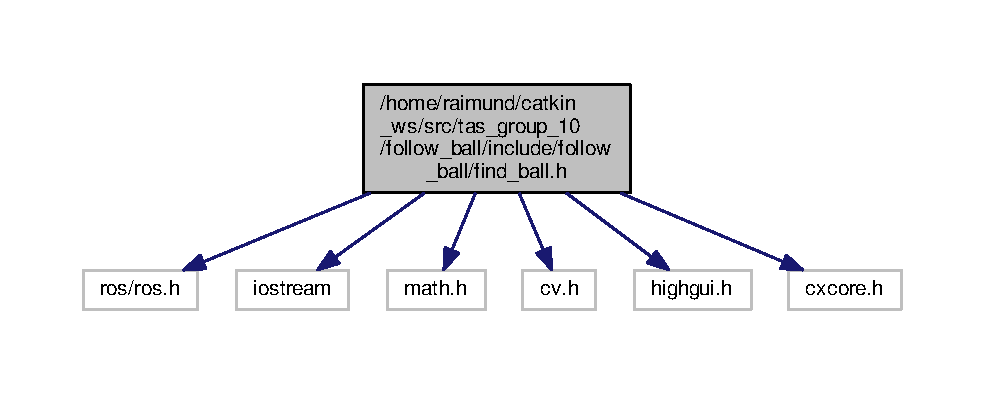
\includegraphics[width=350pt]{find__ball_8h__incl}
\end{center}
\end{figure}
This graph shows which files directly or indirectly include this file\+:
\nopagebreak
\begin{figure}[H]
\begin{center}
\leavevmode
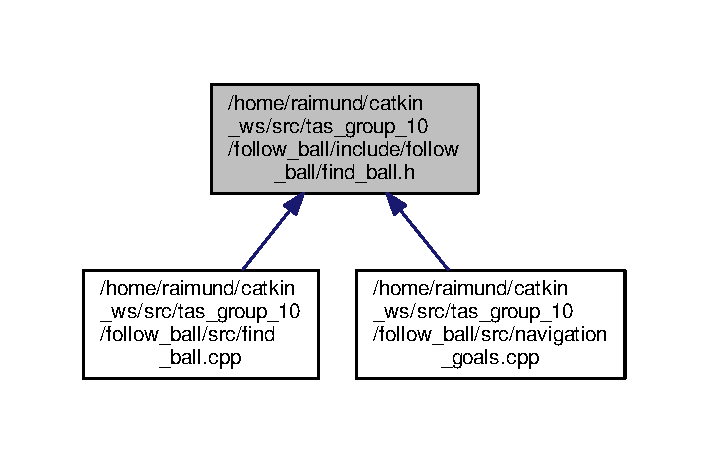
\includegraphics[width=340pt]{find__ball_8h__dep__incl}
\end{center}
\end{figure}
\subsection*{Classes}
\begin{DoxyCompactItemize}
\item 
struct \hyperlink{struct_circle}{Circle}
\item 
class \hyperlink{class_find_ball}{Find\+Ball}
\end{DoxyCompactItemize}
\subsection*{Macros}
\begin{DoxyCompactItemize}
\item 
\#define \hyperlink{find__ball_8h_a9b70b41e2a3d579a874ca76d67eead7f}{S\+A\+V\+E\+\_\+\+C\+I\+R\+C\+L\+E\+S}~20
\begin{DoxyCompactList}\small\item\em how many last circles should be stored \end{DoxyCompactList}\item 
\#define \hyperlink{find__ball_8h_a62fe57ebd3c5b9126fff3612d3e18676}{M\+I\+N\+\_\+\+C\+I\+R\+C\+L\+E\+S}~2
\begin{DoxyCompactList}\small\item\em if used consisten\+Circle, how many of the same circle shall be seen latley \end{DoxyCompactList}\item 
\#define \hyperlink{find__ball_8h_aa907f2f846dab067bec94dc440c328ce}{S\+A\+M\+E\+\_\+\+C\+I\+R\+C\+L\+E\+\_\+\+T\+H\+R\+E\+S\+H\+O\+L\+D}~10
\item 
\#define \hyperlink{find__ball_8h_a2978c2a51c673246e4e319db182270d5}{M\+I\+N\+\_\+\+C\+I\+R\+C\+L\+E\+S\+\_\+\+T\+H\+R\+E\+S\+H\+O\+L\+D}~50
\end{DoxyCompactItemize}


\subsection{Macro Definition Documentation}
\hypertarget{find__ball_8h_a62fe57ebd3c5b9126fff3612d3e18676}{}\index{find\+\_\+ball.\+h@{find\+\_\+ball.\+h}!M\+I\+N\+\_\+\+C\+I\+R\+C\+L\+E\+S@{M\+I\+N\+\_\+\+C\+I\+R\+C\+L\+E\+S}}
\index{M\+I\+N\+\_\+\+C\+I\+R\+C\+L\+E\+S@{M\+I\+N\+\_\+\+C\+I\+R\+C\+L\+E\+S}!find\+\_\+ball.\+h@{find\+\_\+ball.\+h}}
\subsubsection[{M\+I\+N\+\_\+\+C\+I\+R\+C\+L\+E\+S}]{\setlength{\rightskip}{0pt plus 5cm}\#define M\+I\+N\+\_\+\+C\+I\+R\+C\+L\+E\+S~2}\label{find__ball_8h_a62fe57ebd3c5b9126fff3612d3e18676}


if used consisten\+Circle, how many of the same circle shall be seen latley 

\hypertarget{find__ball_8h_a2978c2a51c673246e4e319db182270d5}{}\index{find\+\_\+ball.\+h@{find\+\_\+ball.\+h}!M\+I\+N\+\_\+\+C\+I\+R\+C\+L\+E\+S\+\_\+\+T\+H\+R\+E\+S\+H\+O\+L\+D@{M\+I\+N\+\_\+\+C\+I\+R\+C\+L\+E\+S\+\_\+\+T\+H\+R\+E\+S\+H\+O\+L\+D}}
\index{M\+I\+N\+\_\+\+C\+I\+R\+C\+L\+E\+S\+\_\+\+T\+H\+R\+E\+S\+H\+O\+L\+D@{M\+I\+N\+\_\+\+C\+I\+R\+C\+L\+E\+S\+\_\+\+T\+H\+R\+E\+S\+H\+O\+L\+D}!find\+\_\+ball.\+h@{find\+\_\+ball.\+h}}
\subsubsection[{M\+I\+N\+\_\+\+C\+I\+R\+C\+L\+E\+S\+\_\+\+T\+H\+R\+E\+S\+H\+O\+L\+D}]{\setlength{\rightskip}{0pt plus 5cm}\#define M\+I\+N\+\_\+\+C\+I\+R\+C\+L\+E\+S\+\_\+\+T\+H\+R\+E\+S\+H\+O\+L\+D~50}\label{find__ball_8h_a2978c2a51c673246e4e319db182270d5}
\hypertarget{find__ball_8h_aa907f2f846dab067bec94dc440c328ce}{}\index{find\+\_\+ball.\+h@{find\+\_\+ball.\+h}!S\+A\+M\+E\+\_\+\+C\+I\+R\+C\+L\+E\+\_\+\+T\+H\+R\+E\+S\+H\+O\+L\+D@{S\+A\+M\+E\+\_\+\+C\+I\+R\+C\+L\+E\+\_\+\+T\+H\+R\+E\+S\+H\+O\+L\+D}}
\index{S\+A\+M\+E\+\_\+\+C\+I\+R\+C\+L\+E\+\_\+\+T\+H\+R\+E\+S\+H\+O\+L\+D@{S\+A\+M\+E\+\_\+\+C\+I\+R\+C\+L\+E\+\_\+\+T\+H\+R\+E\+S\+H\+O\+L\+D}!find\+\_\+ball.\+h@{find\+\_\+ball.\+h}}
\subsubsection[{S\+A\+M\+E\+\_\+\+C\+I\+R\+C\+L\+E\+\_\+\+T\+H\+R\+E\+S\+H\+O\+L\+D}]{\setlength{\rightskip}{0pt plus 5cm}\#define S\+A\+M\+E\+\_\+\+C\+I\+R\+C\+L\+E\+\_\+\+T\+H\+R\+E\+S\+H\+O\+L\+D~10}\label{find__ball_8h_aa907f2f846dab067bec94dc440c328ce}
\hypertarget{find__ball_8h_a9b70b41e2a3d579a874ca76d67eead7f}{}\index{find\+\_\+ball.\+h@{find\+\_\+ball.\+h}!S\+A\+V\+E\+\_\+\+C\+I\+R\+C\+L\+E\+S@{S\+A\+V\+E\+\_\+\+C\+I\+R\+C\+L\+E\+S}}
\index{S\+A\+V\+E\+\_\+\+C\+I\+R\+C\+L\+E\+S@{S\+A\+V\+E\+\_\+\+C\+I\+R\+C\+L\+E\+S}!find\+\_\+ball.\+h@{find\+\_\+ball.\+h}}
\subsubsection[{S\+A\+V\+E\+\_\+\+C\+I\+R\+C\+L\+E\+S}]{\setlength{\rightskip}{0pt plus 5cm}\#define S\+A\+V\+E\+\_\+\+C\+I\+R\+C\+L\+E\+S~20}\label{find__ball_8h_a9b70b41e2a3d579a874ca76d67eead7f}


how many last circles should be stored 


\hypertarget{calibrate__params_8cpp}{}\section{/home/raimund/catkin\+\_\+ws/src/tas\+\_\+group\+\_\+10/follow\+\_\+ball/src/calibrate\+\_\+params.cpp File Reference}
\label{calibrate__params_8cpp}\index{/home/raimund/catkin\+\_\+ws/src/tas\+\_\+group\+\_\+10/follow\+\_\+ball/src/calibrate\+\_\+params.\+cpp@{/home/raimund/catkin\+\_\+ws/src/tas\+\_\+group\+\_\+10/follow\+\_\+ball/src/calibrate\+\_\+params.\+cpp}}
{\ttfamily \#include $<$cv.\+h$>$}\\*
{\ttfamily \#include $<$highgui.\+h$>$}\\*
{\ttfamily \#include $<$cxcore.\+h$>$}\\*
{\ttfamily \#include $<$iostream$>$}\\*
Include dependency graph for calibrate\+\_\+params.\+cpp\+:
\nopagebreak
\begin{figure}[H]
\begin{center}
\leavevmode
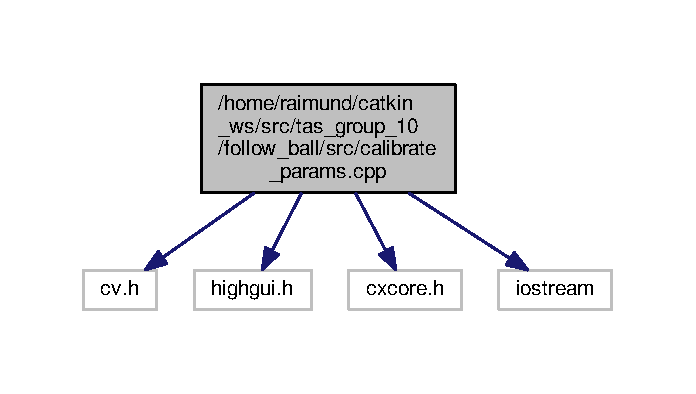
\includegraphics[width=334pt]{calibrate__params_8cpp__incl}
\end{center}
\end{figure}
\subsection*{Functions}
\begin{DoxyCompactItemize}
\item 
void \hyperlink{calibrate__params_8cpp_aae27fc68e5f60017056238857e3b045a}{end} (void) \+\_\+\+\_\+attribute\+\_\+\+\_\+((destructor))
\item 
void \hyperlink{calibrate__params_8cpp_acd0f39dcf5b0ffd24eb1e258857fb739}{on\+\_\+trackbar} (int, void $\ast$)
\item 
int \hyperlink{calibrate__params_8cpp_a0ddf1224851353fc92bfbff6f499fa97}{main} (int argc, char $\ast$argv\mbox{[}$\,$\mbox{]})
\end{DoxyCompactItemize}
\subsection*{Variables}
\begin{DoxyCompactItemize}
\item 
Cv\+Capture $\ast$ \hyperlink{calibrate__params_8cpp_a198bdff9cd5bbbec9c3d248fea2a6101}{capture}
\item 
int \hyperlink{calibrate__params_8cpp_a8ed2fd08b1e388897b555e186ea0f9ff}{device} = 0
\end{DoxyCompactItemize}


\subsection{Function Documentation}
\hypertarget{calibrate__params_8cpp_aae27fc68e5f60017056238857e3b045a}{}\index{calibrate\+\_\+params.\+cpp@{calibrate\+\_\+params.\+cpp}!end@{end}}
\index{end@{end}!calibrate\+\_\+params.\+cpp@{calibrate\+\_\+params.\+cpp}}
\subsubsection[{end}]{\setlength{\rightskip}{0pt plus 5cm}void end (
\begin{DoxyParamCaption}
\item[{void}]{}
\end{DoxyParamCaption}
)}\label{calibrate__params_8cpp_aae27fc68e5f60017056238857e3b045a}
\hypertarget{calibrate__params_8cpp_a0ddf1224851353fc92bfbff6f499fa97}{}\index{calibrate\+\_\+params.\+cpp@{calibrate\+\_\+params.\+cpp}!main@{main}}
\index{main@{main}!calibrate\+\_\+params.\+cpp@{calibrate\+\_\+params.\+cpp}}
\subsubsection[{main}]{\setlength{\rightskip}{0pt plus 5cm}int main (
\begin{DoxyParamCaption}
\item[{int}]{argc, }
\item[{char $\ast$}]{argv\mbox{[}$\,$\mbox{]}}
\end{DoxyParamCaption}
)}\label{calibrate__params_8cpp_a0ddf1224851353fc92bfbff6f499fa97}
\hypertarget{calibrate__params_8cpp_acd0f39dcf5b0ffd24eb1e258857fb739}{}\index{calibrate\+\_\+params.\+cpp@{calibrate\+\_\+params.\+cpp}!on\+\_\+trackbar@{on\+\_\+trackbar}}
\index{on\+\_\+trackbar@{on\+\_\+trackbar}!calibrate\+\_\+params.\+cpp@{calibrate\+\_\+params.\+cpp}}
\subsubsection[{on\+\_\+trackbar}]{\setlength{\rightskip}{0pt plus 5cm}void on\+\_\+trackbar (
\begin{DoxyParamCaption}
\item[{int}]{, }
\item[{void $\ast$}]{}
\end{DoxyParamCaption}
)}\label{calibrate__params_8cpp_acd0f39dcf5b0ffd24eb1e258857fb739}


\subsection{Variable Documentation}
\hypertarget{calibrate__params_8cpp_a198bdff9cd5bbbec9c3d248fea2a6101}{}\index{calibrate\+\_\+params.\+cpp@{calibrate\+\_\+params.\+cpp}!capture@{capture}}
\index{capture@{capture}!calibrate\+\_\+params.\+cpp@{calibrate\+\_\+params.\+cpp}}
\subsubsection[{capture}]{\setlength{\rightskip}{0pt plus 5cm}Cv\+Capture$\ast$ capture}\label{calibrate__params_8cpp_a198bdff9cd5bbbec9c3d248fea2a6101}
\hypertarget{calibrate__params_8cpp_a8ed2fd08b1e388897b555e186ea0f9ff}{}\index{calibrate\+\_\+params.\+cpp@{calibrate\+\_\+params.\+cpp}!device@{device}}
\index{device@{device}!calibrate\+\_\+params.\+cpp@{calibrate\+\_\+params.\+cpp}}
\subsubsection[{device}]{\setlength{\rightskip}{0pt plus 5cm}int device = 0}\label{calibrate__params_8cpp_a8ed2fd08b1e388897b555e186ea0f9ff}

\hypertarget{find__ball_8cpp}{}\section{/home/raimund/catkin\+\_\+ws/src/tas\+\_\+group\+\_\+10/follow\+\_\+ball/src/find\+\_\+ball.cpp File Reference}
\label{find__ball_8cpp}\index{/home/raimund/catkin\+\_\+ws/src/tas\+\_\+group\+\_\+10/follow\+\_\+ball/src/find\+\_\+ball.\+cpp@{/home/raimund/catkin\+\_\+ws/src/tas\+\_\+group\+\_\+10/follow\+\_\+ball/src/find\+\_\+ball.\+cpp}}
{\ttfamily \#include \char`\"{}../include/follow\+\_\+ball/find\+\_\+ball.\+h\char`\"{}}\\*
Include dependency graph for find\+\_\+ball.\+cpp\+:
\nopagebreak
\begin{figure}[H]
\begin{center}
\leavevmode
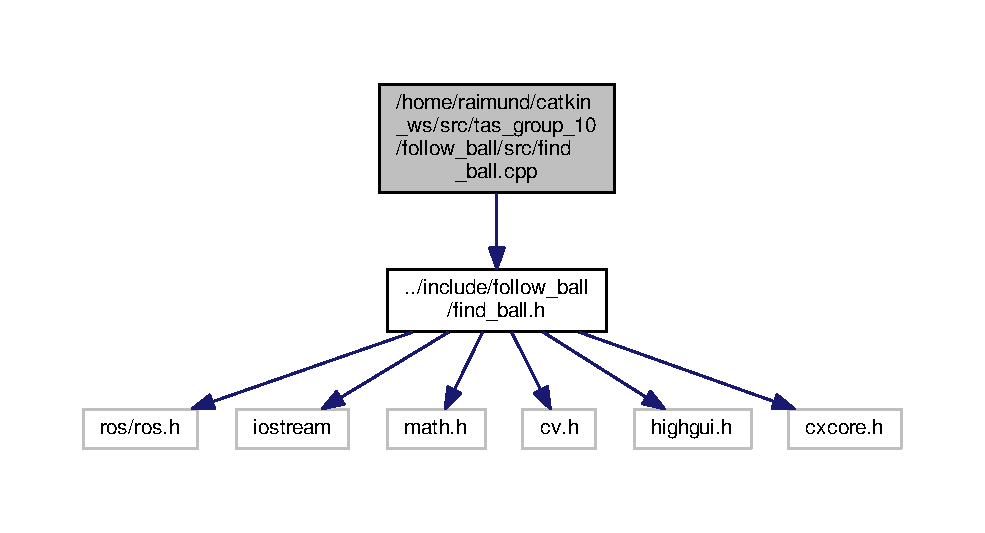
\includegraphics[width=350pt]{find__ball_8cpp__incl}
\end{center}
\end{figure}

\hypertarget{navigation__goals_8cpp}{}\section{/home/raimund/catkin\+\_\+ws/src/tas\+\_\+group\+\_\+10/follow\+\_\+ball/src/navigation\+\_\+goals.cpp File Reference}
\label{navigation__goals_8cpp}\index{/home/raimund/catkin\+\_\+ws/src/tas\+\_\+group\+\_\+10/follow\+\_\+ball/src/navigation\+\_\+goals.\+cpp@{/home/raimund/catkin\+\_\+ws/src/tas\+\_\+group\+\_\+10/follow\+\_\+ball/src/navigation\+\_\+goals.\+cpp}}
{\ttfamily \#include $<$ros/ros.\+h$>$}\\*
{\ttfamily \#include $<$move\+\_\+base\+\_\+msgs/\+Move\+Base\+Action.\+h$>$}\\*
{\ttfamily \#include $<$actionlib/client/simple\+\_\+action\+\_\+client.\+h$>$}\\*
{\ttfamily \#include \char`\"{}../include/follow\+\_\+ball/find\+\_\+ball.\+h\char`\"{}}\\*
{\ttfamily \#include \char`\"{}geometry\+\_\+msgs/\+Vector3.\+h\char`\"{}}\\*
{\ttfamily \#include \char`\"{}sensor\+\_\+msgs/\+Laser\+Scan.\+h\char`\"{}}\\*
{\ttfamily \#include $<$tf/tf.\+h$>$}\\*
{\ttfamily \#include $<$wiimote/\+State.\+h$>$}\\*
{\ttfamily \#include \char`\"{}opencv2/opencv.\+hpp\char`\"{}}\\*
Include dependency graph for navigation\+\_\+goals.\+cpp\+:
\nopagebreak
\begin{figure}[H]
\begin{center}
\leavevmode
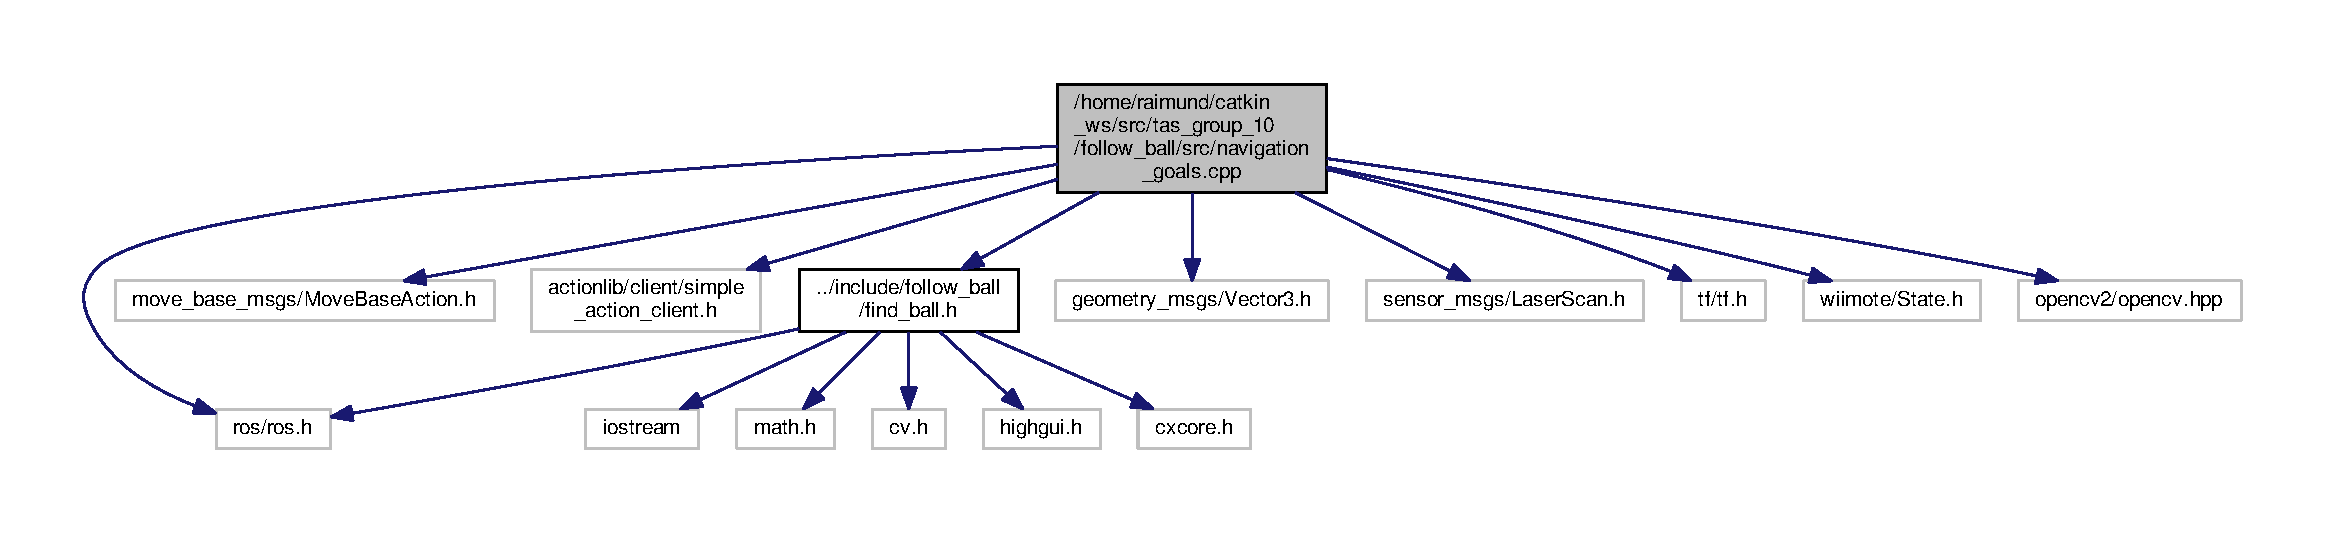
\includegraphics[width=350pt]{navigation__goals_8cpp__incl}
\end{center}
\end{figure}
\subsection*{Macros}
\begin{DoxyCompactItemize}
\item 
\#define \hyperlink{navigation__goals_8cpp_a22a4a74921a4675329f8f987f931f153}{D\+E\+S\+I\+R\+E\+D\+\_\+\+R}~55
\begin{DoxyCompactList}\small\item\em desired radius of the ball in the image \end{DoxyCompactList}\item 
\#define \hyperlink{navigation__goals_8cpp_afc1e832a8c33311f4ca0feb53dbe3c54}{D\+E\+S\+I\+R\+E\+D\+\_\+\+Y}~3/4
\begin{DoxyCompactList}\small\item\em desired Y-\/coordinate of the center of the ball, if higher, go backwards (ball at the bottom of the image \end{DoxyCompactList}\item 
\#define \hyperlink{navigation__goals_8cpp_a4fb9a482de80f37e77695daa1d38e548}{N\+U\+M\+B\+E\+R\+\_\+\+I\+N\+T}~10
\begin{DoxyCompactList}\small\item\em how many steps should be saved for the integral part of the pid controller \end{DoxyCompactList}\item 
\#define \hyperlink{navigation__goals_8cpp_aa4729260b732666338dee7d841aa12f3}{K\+P}~1.\+0
\begin{DoxyCompactList}\small\item\em value for P\+I\+D controller (using r value of circle to track distance) \end{DoxyCompactList}\item 
\#define \hyperlink{navigation__goals_8cpp_ade82752ae1652fdf0df9df7a16ffda29}{K\+I}~2/\hyperlink{navigation__goals_8cpp_a4fb9a482de80f37e77695daa1d38e548}{N\+U\+M\+B\+E\+R\+\_\+\+I\+N\+T}
\begin{DoxyCompactList}\small\item\em values for P\+I\+D controller (using r value of circle to track distance) \end{DoxyCompactList}\item 
\#define \hyperlink{navigation__goals_8cpp_ad4f9673d16d231643789f081068d2372}{K\+D}~0.\+5
\begin{DoxyCompactList}\small\item\em values for P\+I\+D controller (using r value of circle to track distance) \end{DoxyCompactList}\item 
\#define \hyperlink{navigation__goals_8cpp_a83f074e666632431ae6d34eed35d5fe9}{K\+P\+Y}~-\/1/4
\begin{DoxyCompactList}\small\item\em value for P controller (using y koordinate to track distance) \end{DoxyCompactList}\item 
\#define \hyperlink{navigation__goals_8cpp_a9f6b452e529861368b0acfd411437c71}{A\+N\+G\+L\+E\+\_\+\+M\+A\+X}~M\+\_\+\+P\+I\+\_\+4
\begin{DoxyCompactList}\small\item\em max angle of camera (add a bit so it follows more than it should) \end{DoxyCompactList}\item 
\#define \hyperlink{navigation__goals_8cpp_af0f97ec9692f26180727c94af51cfedc}{O\+A}~0.\+5
\begin{DoxyCompactList}\small\item\em orientation controller is quadratic, it trys way harder if the ball is at the edge of the image (O\+A$\ast$xdiff² + O\+B$\ast$xdiff) \end{DoxyCompactList}\item 
\#define \hyperlink{navigation__goals_8cpp_ad2d5f875cdc6d696735f20fa23a895c3}{O\+B}~1
\begin{DoxyCompactList}\small\item\em orientation controller is quadratic, it trys way harder if the ball is at the edge of the image (O\+A$\ast$xdiff² + O\+B$\ast$xdiff) \end{DoxyCompactList}\item 
\#define \hyperlink{navigation__goals_8cpp_a3c983eeadd733105fb0fea8729a9f2db}{R\+A\+N\+G\+E\+\_\+\+M\+I\+N}~0.\+12
\begin{DoxyCompactList}\small\item\em range which should stop movement \end{DoxyCompactList}\item 
\#define \hyperlink{navigation__goals_8cpp_adf268402c73f6701eef6c494ecfacb30}{M\+A\+X\+\_\+\+S\+E\+C\+\_\+\+T\+R\+Y\+\_\+\+T\+O\+\_\+\+F\+O\+L\+L\+O\+W}~2
\begin{DoxyCompactList}\small\item\em time it should try to follow \end{DoxyCompactList}\item 
\#define \hyperlink{navigation__goals_8cpp_a906a40b0c527739a26ef013ac36157cb}{W\+I\+I\+\_\+\+B\+U\+T\+T\+O\+N\+\_\+\+N\+U\+N\+C\+H\+U\+K\+\_\+\+C}~1
\end{DoxyCompactItemize}
\subsection*{Typedefs}
\begin{DoxyCompactItemize}
\item 
typedef actionlib\+::\+Simple\+Action\+Client$<$ move\+\_\+base\+\_\+msgs\+::\+Move\+Base\+Action $>$ \hyperlink{navigation__goals_8cpp_a21e20cc0b6656ae897b3cbb969b93241}{Move\+Base\+Client}
\end{DoxyCompactItemize}
\subsection*{Functions}
\begin{DoxyCompactItemize}
\item 
geometry\+\_\+msgs\+::\+Vector3 \hyperlink{navigation__goals_8cpp_afc95d0744af55570d5f72e2c007d26b1}{build\+\_\+servo} (double linear, double orientation)
\begin{DoxyCompactList}\small\item\em build\+\_\+servo builds servo-\/message with respect to linear and orientation \end{DoxyCompactList}\item 
move\+\_\+base\+\_\+msgs\+::\+Move\+Base\+Goal \hyperlink{navigation__goals_8cpp_a098ab7cdd714d111e73008cf0697451e}{build\+\_\+goal} (double linear, double orientation)
\begin{DoxyCompactList}\small\item\em build\+\_\+goal builds move\+\_\+baseage with respect to linear and orientation \end{DoxyCompactList}\item 
double \hyperlink{navigation__goals_8cpp_ad5f77055f741363f57129694d8359928}{get\+\_\+linear\+\_\+goal\+\_\+y} (\hyperlink{struct_circle}{Circle} circle)
\begin{DoxyCompactList}\small\item\em get\+\_\+linear\+\_\+goal\+\_\+y builds linear speed with respect to the y-\/coordinate of the center of the circle \end{DoxyCompactList}\item 
double \hyperlink{navigation__goals_8cpp_aee50875eee1021ae02124e589a3d2ca0}{get\+\_\+linear\+\_\+goal} (\hyperlink{struct_circle}{Circle} circle)
\begin{DoxyCompactList}\small\item\em get\+\_\+linear\+\_\+goal builds linear speed with respect to the radius of the circle \end{DoxyCompactList}\item 
double \hyperlink{navigation__goals_8cpp_ad77bcfe20d953822874ffb11f2b4c2ed}{get\+\_\+orientation} (\hyperlink{struct_circle}{Circle} circle)
\begin{DoxyCompactList}\small\item\em get\+\_\+orientation builds orientation with respect to the x-\/coordinate of the center of the circle \end{DoxyCompactList}\item 
void \hyperlink{navigation__goals_8cpp_a401b97abbf3e813f2981b210379b4908}{wii\+Callback} (const wiimote\+::\+State\+::\+Const\+Ptr \&wii\+State)
\begin{DoxyCompactList}\small\item\em wii\+Callback callback for wii-\/controller, sets nunchuk\+\_\+c\+\_\+pressed \end{DoxyCompactList}\item 
void \hyperlink{navigation__goals_8cpp_adc74481f7eae4505d3200f9f128c4744}{scan\+Callback} (const sensor\+\_\+msgs\+::\+Laser\+Scan\+Const\+Ptr \&scan)
\item 
int \hyperlink{navigation__goals_8cpp_a3c04138a5bfe5d72780bb7e82a18e627}{main} (int argc, char $\ast$$\ast$argv)
\end{DoxyCompactItemize}
\subsection*{Variables}
\begin{DoxyCompactItemize}
\item 
bool \hyperlink{navigation__goals_8cpp_a53a2d16dac430353052f49aaa0cce34a}{stop} = false
\begin{DoxyCompactList}\small\item\em stop if near a wall \end{DoxyCompactList}\item 
int \hyperlink{navigation__goals_8cpp_a86cf672daa4e0ad11ad10efc894d19c8}{num} = 0
\begin{DoxyCompactList}\small\item\em seq number of goal for autonomous driving \end{DoxyCompactList}\item 
double \hyperlink{navigation__goals_8cpp_a6943d822a23db3c821ac66e3482e09f5}{desired\+\_\+x} = 0
\begin{DoxyCompactList}\small\item\em corresponce to the middlepoint of the image \end{DoxyCompactList}\item 
double \hyperlink{navigation__goals_8cpp_aa094a11625b9bf726abdb71caed8c9f1}{desired\+\_\+y} = 0
\begin{DoxyCompactList}\small\item\em corresponce to D\+E\+S\+I\+R\+E\+D\+\_\+\+Y \end{DoxyCompactList}\item 
std\+::vector$<$ double $>$ \hyperlink{navigation__goals_8cpp_a88864b29831db214ef58148acf0b8db4}{linear\+\_\+int}
\begin{DoxyCompactList}\small\item\em Array for the Integral-\/\+Part of the P\+I\+D Controller. \end{DoxyCompactList}\item 
int \hyperlink{navigation__goals_8cpp_a084d89d497823f129f42ae61662efee4}{linear\+\_\+int\+\_\+idx} = 0
\begin{DoxyCompactList}\small\item\em current index of lienar\+\_\+int \end{DoxyCompactList}\item 
bool \hyperlink{navigation__goals_8cpp_a5bafc98f16f9fd53e0f929fe20b17e1c}{show} = false
\begin{DoxyCompactList}\small\item\em should the images be shown on screen? \end{DoxyCompactList}\item 
bool \hyperlink{navigation__goals_8cpp_a4a4c92bfaf637dd8d1776e2ed78dded5}{use\+\_\+autonomus} = false
\begin{DoxyCompactList}\small\item\em should it use autnomous driving (send goals) or try to follow directly (send servo commands) !\+W\+A\+R\+N\+I\+N\+G -\/$>$ no avoiding! Only drives while Nunchuck button C is pressed \end{DoxyCompactList}\item 
bool \hyperlink{navigation__goals_8cpp_aa8828b6f9054e8ce4fa719f5790f0ad7}{nunchuk\+\_\+c\+\_\+pressed} = false
\begin{DoxyCompactList}\small\item\em value to tell if nunchuk c is pressed \end{DoxyCompactList}\item 
double \hyperlink{navigation__goals_8cpp_aaed5ad0eb2165b9cd4b804f12f44f624}{last\+\_\+orientation} = 0
\begin{DoxyCompactList}\small\item\em last orientation value to try to follow if not autonomous driving is used \end{DoxyCompactList}\item 
double \hyperlink{navigation__goals_8cpp_ae432752a3c95315a00b3e3b42d4ba468}{last\+\_\+linear} = 0
\begin{DoxyCompactList}\small\item\em last linear value \end{DoxyCompactList}\item 
int \hyperlink{navigation__goals_8cpp_a41c2f8914d0edbc9bfe8019697280a82}{counter\+\_\+try\+\_\+to\+\_\+follow} = 0
\begin{DoxyCompactList}\small\item\em counter so it doesnt try to follow forever \end{DoxyCompactList}\item 
int \hyperlink{navigation__goals_8cpp_aea95c33791f3b1d4c3db490749dcc4c2}{counter\+\_\+back} = 0
\begin{DoxyCompactList}\small\item\em counter so it actually drives backwards \end{DoxyCompactList}\end{DoxyCompactItemize}


\subsection{Macro Definition Documentation}
\hypertarget{navigation__goals_8cpp_a9f6b452e529861368b0acfd411437c71}{}\index{navigation\+\_\+goals.\+cpp@{navigation\+\_\+goals.\+cpp}!A\+N\+G\+L\+E\+\_\+\+M\+A\+X@{A\+N\+G\+L\+E\+\_\+\+M\+A\+X}}
\index{A\+N\+G\+L\+E\+\_\+\+M\+A\+X@{A\+N\+G\+L\+E\+\_\+\+M\+A\+X}!navigation\+\_\+goals.\+cpp@{navigation\+\_\+goals.\+cpp}}
\subsubsection[{A\+N\+G\+L\+E\+\_\+\+M\+A\+X}]{\setlength{\rightskip}{0pt plus 5cm}\#define A\+N\+G\+L\+E\+\_\+\+M\+A\+X~M\+\_\+\+P\+I\+\_\+4}\label{navigation__goals_8cpp_a9f6b452e529861368b0acfd411437c71}


max angle of camera (add a bit so it follows more than it should) 

\hypertarget{navigation__goals_8cpp_a22a4a74921a4675329f8f987f931f153}{}\index{navigation\+\_\+goals.\+cpp@{navigation\+\_\+goals.\+cpp}!D\+E\+S\+I\+R\+E\+D\+\_\+\+R@{D\+E\+S\+I\+R\+E\+D\+\_\+\+R}}
\index{D\+E\+S\+I\+R\+E\+D\+\_\+\+R@{D\+E\+S\+I\+R\+E\+D\+\_\+\+R}!navigation\+\_\+goals.\+cpp@{navigation\+\_\+goals.\+cpp}}
\subsubsection[{D\+E\+S\+I\+R\+E\+D\+\_\+\+R}]{\setlength{\rightskip}{0pt plus 5cm}\#define D\+E\+S\+I\+R\+E\+D\+\_\+\+R~55}\label{navigation__goals_8cpp_a22a4a74921a4675329f8f987f931f153}


desired radius of the ball in the image 

\hypertarget{navigation__goals_8cpp_afc1e832a8c33311f4ca0feb53dbe3c54}{}\index{navigation\+\_\+goals.\+cpp@{navigation\+\_\+goals.\+cpp}!D\+E\+S\+I\+R\+E\+D\+\_\+\+Y@{D\+E\+S\+I\+R\+E\+D\+\_\+\+Y}}
\index{D\+E\+S\+I\+R\+E\+D\+\_\+\+Y@{D\+E\+S\+I\+R\+E\+D\+\_\+\+Y}!navigation\+\_\+goals.\+cpp@{navigation\+\_\+goals.\+cpp}}
\subsubsection[{D\+E\+S\+I\+R\+E\+D\+\_\+\+Y}]{\setlength{\rightskip}{0pt plus 5cm}\#define D\+E\+S\+I\+R\+E\+D\+\_\+\+Y~3/4}\label{navigation__goals_8cpp_afc1e832a8c33311f4ca0feb53dbe3c54}


desired Y-\/coordinate of the center of the ball, if higher, go backwards (ball at the bottom of the image 

\hypertarget{navigation__goals_8cpp_ad4f9673d16d231643789f081068d2372}{}\index{navigation\+\_\+goals.\+cpp@{navigation\+\_\+goals.\+cpp}!K\+D@{K\+D}}
\index{K\+D@{K\+D}!navigation\+\_\+goals.\+cpp@{navigation\+\_\+goals.\+cpp}}
\subsubsection[{K\+D}]{\setlength{\rightskip}{0pt plus 5cm}\#define K\+D~0.\+5}\label{navigation__goals_8cpp_ad4f9673d16d231643789f081068d2372}


values for P\+I\+D controller (using r value of circle to track distance) 

\hypertarget{navigation__goals_8cpp_ade82752ae1652fdf0df9df7a16ffda29}{}\index{navigation\+\_\+goals.\+cpp@{navigation\+\_\+goals.\+cpp}!K\+I@{K\+I}}
\index{K\+I@{K\+I}!navigation\+\_\+goals.\+cpp@{navigation\+\_\+goals.\+cpp}}
\subsubsection[{K\+I}]{\setlength{\rightskip}{0pt plus 5cm}\#define K\+I~2/{\bf N\+U\+M\+B\+E\+R\+\_\+\+I\+N\+T}}\label{navigation__goals_8cpp_ade82752ae1652fdf0df9df7a16ffda29}


values for P\+I\+D controller (using r value of circle to track distance) 

\hypertarget{navigation__goals_8cpp_aa4729260b732666338dee7d841aa12f3}{}\index{navigation\+\_\+goals.\+cpp@{navigation\+\_\+goals.\+cpp}!K\+P@{K\+P}}
\index{K\+P@{K\+P}!navigation\+\_\+goals.\+cpp@{navigation\+\_\+goals.\+cpp}}
\subsubsection[{K\+P}]{\setlength{\rightskip}{0pt plus 5cm}\#define K\+P~1.\+0}\label{navigation__goals_8cpp_aa4729260b732666338dee7d841aa12f3}


value for P\+I\+D controller (using r value of circle to track distance) 

\hypertarget{navigation__goals_8cpp_a83f074e666632431ae6d34eed35d5fe9}{}\index{navigation\+\_\+goals.\+cpp@{navigation\+\_\+goals.\+cpp}!K\+P\+Y@{K\+P\+Y}}
\index{K\+P\+Y@{K\+P\+Y}!navigation\+\_\+goals.\+cpp@{navigation\+\_\+goals.\+cpp}}
\subsubsection[{K\+P\+Y}]{\setlength{\rightskip}{0pt plus 5cm}\#define K\+P\+Y~-\/1/4}\label{navigation__goals_8cpp_a83f074e666632431ae6d34eed35d5fe9}


value for P controller (using y koordinate to track distance) 

\hypertarget{navigation__goals_8cpp_adf268402c73f6701eef6c494ecfacb30}{}\index{navigation\+\_\+goals.\+cpp@{navigation\+\_\+goals.\+cpp}!M\+A\+X\+\_\+\+S\+E\+C\+\_\+\+T\+R\+Y\+\_\+\+T\+O\+\_\+\+F\+O\+L\+L\+O\+W@{M\+A\+X\+\_\+\+S\+E\+C\+\_\+\+T\+R\+Y\+\_\+\+T\+O\+\_\+\+F\+O\+L\+L\+O\+W}}
\index{M\+A\+X\+\_\+\+S\+E\+C\+\_\+\+T\+R\+Y\+\_\+\+T\+O\+\_\+\+F\+O\+L\+L\+O\+W@{M\+A\+X\+\_\+\+S\+E\+C\+\_\+\+T\+R\+Y\+\_\+\+T\+O\+\_\+\+F\+O\+L\+L\+O\+W}!navigation\+\_\+goals.\+cpp@{navigation\+\_\+goals.\+cpp}}
\subsubsection[{M\+A\+X\+\_\+\+S\+E\+C\+\_\+\+T\+R\+Y\+\_\+\+T\+O\+\_\+\+F\+O\+L\+L\+O\+W}]{\setlength{\rightskip}{0pt plus 5cm}\#define M\+A\+X\+\_\+\+S\+E\+C\+\_\+\+T\+R\+Y\+\_\+\+T\+O\+\_\+\+F\+O\+L\+L\+O\+W~2}\label{navigation__goals_8cpp_adf268402c73f6701eef6c494ecfacb30}


time it should try to follow 

\hypertarget{navigation__goals_8cpp_a4fb9a482de80f37e77695daa1d38e548}{}\index{navigation\+\_\+goals.\+cpp@{navigation\+\_\+goals.\+cpp}!N\+U\+M\+B\+E\+R\+\_\+\+I\+N\+T@{N\+U\+M\+B\+E\+R\+\_\+\+I\+N\+T}}
\index{N\+U\+M\+B\+E\+R\+\_\+\+I\+N\+T@{N\+U\+M\+B\+E\+R\+\_\+\+I\+N\+T}!navigation\+\_\+goals.\+cpp@{navigation\+\_\+goals.\+cpp}}
\subsubsection[{N\+U\+M\+B\+E\+R\+\_\+\+I\+N\+T}]{\setlength{\rightskip}{0pt plus 5cm}\#define N\+U\+M\+B\+E\+R\+\_\+\+I\+N\+T~10}\label{navigation__goals_8cpp_a4fb9a482de80f37e77695daa1d38e548}


how many steps should be saved for the integral part of the pid controller 

\hypertarget{navigation__goals_8cpp_af0f97ec9692f26180727c94af51cfedc}{}\index{navigation\+\_\+goals.\+cpp@{navigation\+\_\+goals.\+cpp}!O\+A@{O\+A}}
\index{O\+A@{O\+A}!navigation\+\_\+goals.\+cpp@{navigation\+\_\+goals.\+cpp}}
\subsubsection[{O\+A}]{\setlength{\rightskip}{0pt plus 5cm}\#define O\+A~0.\+5}\label{navigation__goals_8cpp_af0f97ec9692f26180727c94af51cfedc}


orientation controller is quadratic, it trys way harder if the ball is at the edge of the image (O\+A$\ast$xdiff² + O\+B$\ast$xdiff) 

\hypertarget{navigation__goals_8cpp_ad2d5f875cdc6d696735f20fa23a895c3}{}\index{navigation\+\_\+goals.\+cpp@{navigation\+\_\+goals.\+cpp}!O\+B@{O\+B}}
\index{O\+B@{O\+B}!navigation\+\_\+goals.\+cpp@{navigation\+\_\+goals.\+cpp}}
\subsubsection[{O\+B}]{\setlength{\rightskip}{0pt plus 5cm}\#define O\+B~1}\label{navigation__goals_8cpp_ad2d5f875cdc6d696735f20fa23a895c3}


orientation controller is quadratic, it trys way harder if the ball is at the edge of the image (O\+A$\ast$xdiff² + O\+B$\ast$xdiff) 

\hypertarget{navigation__goals_8cpp_a3c983eeadd733105fb0fea8729a9f2db}{}\index{navigation\+\_\+goals.\+cpp@{navigation\+\_\+goals.\+cpp}!R\+A\+N\+G\+E\+\_\+\+M\+I\+N@{R\+A\+N\+G\+E\+\_\+\+M\+I\+N}}
\index{R\+A\+N\+G\+E\+\_\+\+M\+I\+N@{R\+A\+N\+G\+E\+\_\+\+M\+I\+N}!navigation\+\_\+goals.\+cpp@{navigation\+\_\+goals.\+cpp}}
\subsubsection[{R\+A\+N\+G\+E\+\_\+\+M\+I\+N}]{\setlength{\rightskip}{0pt plus 5cm}\#define R\+A\+N\+G\+E\+\_\+\+M\+I\+N~0.\+12}\label{navigation__goals_8cpp_a3c983eeadd733105fb0fea8729a9f2db}


range which should stop movement 

\hypertarget{navigation__goals_8cpp_a906a40b0c527739a26ef013ac36157cb}{}\index{navigation\+\_\+goals.\+cpp@{navigation\+\_\+goals.\+cpp}!W\+I\+I\+\_\+\+B\+U\+T\+T\+O\+N\+\_\+\+N\+U\+N\+C\+H\+U\+K\+\_\+\+C@{W\+I\+I\+\_\+\+B\+U\+T\+T\+O\+N\+\_\+\+N\+U\+N\+C\+H\+U\+K\+\_\+\+C}}
\index{W\+I\+I\+\_\+\+B\+U\+T\+T\+O\+N\+\_\+\+N\+U\+N\+C\+H\+U\+K\+\_\+\+C@{W\+I\+I\+\_\+\+B\+U\+T\+T\+O\+N\+\_\+\+N\+U\+N\+C\+H\+U\+K\+\_\+\+C}!navigation\+\_\+goals.\+cpp@{navigation\+\_\+goals.\+cpp}}
\subsubsection[{W\+I\+I\+\_\+\+B\+U\+T\+T\+O\+N\+\_\+\+N\+U\+N\+C\+H\+U\+K\+\_\+\+C}]{\setlength{\rightskip}{0pt plus 5cm}\#define W\+I\+I\+\_\+\+B\+U\+T\+T\+O\+N\+\_\+\+N\+U\+N\+C\+H\+U\+K\+\_\+\+C~1}\label{navigation__goals_8cpp_a906a40b0c527739a26ef013ac36157cb}


\subsection{Typedef Documentation}
\hypertarget{navigation__goals_8cpp_a21e20cc0b6656ae897b3cbb969b93241}{}\index{navigation\+\_\+goals.\+cpp@{navigation\+\_\+goals.\+cpp}!Move\+Base\+Client@{Move\+Base\+Client}}
\index{Move\+Base\+Client@{Move\+Base\+Client}!navigation\+\_\+goals.\+cpp@{navigation\+\_\+goals.\+cpp}}
\subsubsection[{Move\+Base\+Client}]{\setlength{\rightskip}{0pt plus 5cm}typedef actionlib\+::\+Simple\+Action\+Client$<$move\+\_\+base\+\_\+msgs\+::\+Move\+Base\+Action$>$ {\bf Move\+Base\+Client}}\label{navigation__goals_8cpp_a21e20cc0b6656ae897b3cbb969b93241}


\subsection{Function Documentation}
\hypertarget{navigation__goals_8cpp_a098ab7cdd714d111e73008cf0697451e}{}\index{navigation\+\_\+goals.\+cpp@{navigation\+\_\+goals.\+cpp}!build\+\_\+goal@{build\+\_\+goal}}
\index{build\+\_\+goal@{build\+\_\+goal}!navigation\+\_\+goals.\+cpp@{navigation\+\_\+goals.\+cpp}}
\subsubsection[{build\+\_\+goal}]{\setlength{\rightskip}{0pt plus 5cm}move\+\_\+base\+\_\+msgs\+::\+Move\+Base\+Goal build\+\_\+goal (
\begin{DoxyParamCaption}
\item[{double}]{linear, }
\item[{double}]{orientation}
\end{DoxyParamCaption}
)}\label{navigation__goals_8cpp_a098ab7cdd714d111e73008cf0697451e}


build\+\_\+goal builds move\+\_\+baseage with respect to linear and orientation 


\begin{DoxyParams}{Parameters}
{\em linear} & positiv if it should drive forward, near 0 if it should stop, negativ if drive backwards \\
\hline
{\em orientation} & orientation if it should drive left or right \\
\hline
\end{DoxyParams}
\begin{DoxyReturn}{Returns}
move\+\_\+base message which should be published to /move\+\_\+base\+\_\+simple/goal 
\end{DoxyReturn}
\hypertarget{navigation__goals_8cpp_afc95d0744af55570d5f72e2c007d26b1}{}\index{navigation\+\_\+goals.\+cpp@{navigation\+\_\+goals.\+cpp}!build\+\_\+servo@{build\+\_\+servo}}
\index{build\+\_\+servo@{build\+\_\+servo}!navigation\+\_\+goals.\+cpp@{navigation\+\_\+goals.\+cpp}}
\subsubsection[{build\+\_\+servo}]{\setlength{\rightskip}{0pt plus 5cm}geometry\+\_\+msgs\+::\+Vector3 build\+\_\+servo (
\begin{DoxyParamCaption}
\item[{double}]{linear, }
\item[{double}]{orientation}
\end{DoxyParamCaption}
)}\label{navigation__goals_8cpp_afc95d0744af55570d5f72e2c007d26b1}


build\+\_\+servo builds servo-\/message with respect to linear and orientation 


\begin{DoxyParams}{Parameters}
{\em linear} & positiv if it should drive forward, near 0 if it should stop, negativ if drive backwards \\
\hline
{\em orientation} & orientation if it should drive left or right \\
\hline
\end{DoxyParams}
\begin{DoxyReturn}{Returns}
servo-\/message which should be published to /servo 
\end{DoxyReturn}
\hypertarget{navigation__goals_8cpp_aee50875eee1021ae02124e589a3d2ca0}{}\index{navigation\+\_\+goals.\+cpp@{navigation\+\_\+goals.\+cpp}!get\+\_\+linear\+\_\+goal@{get\+\_\+linear\+\_\+goal}}
\index{get\+\_\+linear\+\_\+goal@{get\+\_\+linear\+\_\+goal}!navigation\+\_\+goals.\+cpp@{navigation\+\_\+goals.\+cpp}}
\subsubsection[{get\+\_\+linear\+\_\+goal}]{\setlength{\rightskip}{0pt plus 5cm}double get\+\_\+linear\+\_\+goal (
\begin{DoxyParamCaption}
\item[{{\bf Circle}}]{circle}
\end{DoxyParamCaption}
)}\label{navigation__goals_8cpp_aee50875eee1021ae02124e589a3d2ca0}


get\+\_\+linear\+\_\+goal builds linear speed with respect to the radius of the circle 


\begin{DoxyParams}{Parameters}
{\em circle} & circle which shall be followed \\
\hline
\end{DoxyParams}
\begin{DoxyReturn}{Returns}
linear speed 
\end{DoxyReturn}
\hypertarget{navigation__goals_8cpp_ad5f77055f741363f57129694d8359928}{}\index{navigation\+\_\+goals.\+cpp@{navigation\+\_\+goals.\+cpp}!get\+\_\+linear\+\_\+goal\+\_\+y@{get\+\_\+linear\+\_\+goal\+\_\+y}}
\index{get\+\_\+linear\+\_\+goal\+\_\+y@{get\+\_\+linear\+\_\+goal\+\_\+y}!navigation\+\_\+goals.\+cpp@{navigation\+\_\+goals.\+cpp}}
\subsubsection[{get\+\_\+linear\+\_\+goal\+\_\+y}]{\setlength{\rightskip}{0pt plus 5cm}double get\+\_\+linear\+\_\+goal\+\_\+y (
\begin{DoxyParamCaption}
\item[{{\bf Circle}}]{circle}
\end{DoxyParamCaption}
)}\label{navigation__goals_8cpp_ad5f77055f741363f57129694d8359928}


get\+\_\+linear\+\_\+goal\+\_\+y builds linear speed with respect to the y-\/coordinate of the center of the circle 


\begin{DoxyParams}{Parameters}
{\em circle} & circle which shall be followed \\
\hline
\end{DoxyParams}
\begin{DoxyReturn}{Returns}
linear speed 
\end{DoxyReturn}
\hypertarget{navigation__goals_8cpp_ad77bcfe20d953822874ffb11f2b4c2ed}{}\index{navigation\+\_\+goals.\+cpp@{navigation\+\_\+goals.\+cpp}!get\+\_\+orientation@{get\+\_\+orientation}}
\index{get\+\_\+orientation@{get\+\_\+orientation}!navigation\+\_\+goals.\+cpp@{navigation\+\_\+goals.\+cpp}}
\subsubsection[{get\+\_\+orientation}]{\setlength{\rightskip}{0pt plus 5cm}double get\+\_\+orientation (
\begin{DoxyParamCaption}
\item[{{\bf Circle}}]{circle}
\end{DoxyParamCaption}
)}\label{navigation__goals_8cpp_ad77bcfe20d953822874ffb11f2b4c2ed}


get\+\_\+orientation builds orientation with respect to the x-\/coordinate of the center of the circle 


\begin{DoxyParams}{Parameters}
{\em circle} & circle which shall be followed \\
\hline
\end{DoxyParams}
\begin{DoxyReturn}{Returns}
orientation which shall be achieved 
\end{DoxyReturn}
\hypertarget{navigation__goals_8cpp_a3c04138a5bfe5d72780bb7e82a18e627}{}\index{navigation\+\_\+goals.\+cpp@{navigation\+\_\+goals.\+cpp}!main@{main}}
\index{main@{main}!navigation\+\_\+goals.\+cpp@{navigation\+\_\+goals.\+cpp}}
\subsubsection[{main}]{\setlength{\rightskip}{0pt plus 5cm}int main (
\begin{DoxyParamCaption}
\item[{int}]{argc, }
\item[{char $\ast$$\ast$}]{argv}
\end{DoxyParamCaption}
)}\label{navigation__goals_8cpp_a3c04138a5bfe5d72780bb7e82a18e627}
\hypertarget{navigation__goals_8cpp_adc74481f7eae4505d3200f9f128c4744}{}\index{navigation\+\_\+goals.\+cpp@{navigation\+\_\+goals.\+cpp}!scan\+Callback@{scan\+Callback}}
\index{scan\+Callback@{scan\+Callback}!navigation\+\_\+goals.\+cpp@{navigation\+\_\+goals.\+cpp}}
\subsubsection[{scan\+Callback}]{\setlength{\rightskip}{0pt plus 5cm}void scan\+Callback (
\begin{DoxyParamCaption}
\item[{const sensor\+\_\+msgs\+::\+Laser\+Scan\+Const\+Ptr \&}]{scan}
\end{DoxyParamCaption}
)}\label{navigation__goals_8cpp_adc74481f7eae4505d3200f9f128c4744}
\hypertarget{navigation__goals_8cpp_a401b97abbf3e813f2981b210379b4908}{}\index{navigation\+\_\+goals.\+cpp@{navigation\+\_\+goals.\+cpp}!wii\+Callback@{wii\+Callback}}
\index{wii\+Callback@{wii\+Callback}!navigation\+\_\+goals.\+cpp@{navigation\+\_\+goals.\+cpp}}
\subsubsection[{wii\+Callback}]{\setlength{\rightskip}{0pt plus 5cm}void wii\+Callback (
\begin{DoxyParamCaption}
\item[{const wiimote\+::\+State\+::\+Const\+Ptr \&}]{wii\+State}
\end{DoxyParamCaption}
)}\label{navigation__goals_8cpp_a401b97abbf3e813f2981b210379b4908}


wii\+Callback callback for wii-\/controller, sets nunchuk\+\_\+c\+\_\+pressed 


\begin{DoxyParams}{Parameters}
{\em wii\+State} & state of the wii-\/controller \\
\hline
\end{DoxyParams}


\subsection{Variable Documentation}
\hypertarget{navigation__goals_8cpp_aea95c33791f3b1d4c3db490749dcc4c2}{}\index{navigation\+\_\+goals.\+cpp@{navigation\+\_\+goals.\+cpp}!counter\+\_\+back@{counter\+\_\+back}}
\index{counter\+\_\+back@{counter\+\_\+back}!navigation\+\_\+goals.\+cpp@{navigation\+\_\+goals.\+cpp}}
\subsubsection[{counter\+\_\+back}]{\setlength{\rightskip}{0pt plus 5cm}int counter\+\_\+back = 0}\label{navigation__goals_8cpp_aea95c33791f3b1d4c3db490749dcc4c2}


counter so it actually drives backwards 

\hypertarget{navigation__goals_8cpp_a41c2f8914d0edbc9bfe8019697280a82}{}\index{navigation\+\_\+goals.\+cpp@{navigation\+\_\+goals.\+cpp}!counter\+\_\+try\+\_\+to\+\_\+follow@{counter\+\_\+try\+\_\+to\+\_\+follow}}
\index{counter\+\_\+try\+\_\+to\+\_\+follow@{counter\+\_\+try\+\_\+to\+\_\+follow}!navigation\+\_\+goals.\+cpp@{navigation\+\_\+goals.\+cpp}}
\subsubsection[{counter\+\_\+try\+\_\+to\+\_\+follow}]{\setlength{\rightskip}{0pt plus 5cm}int counter\+\_\+try\+\_\+to\+\_\+follow = 0}\label{navigation__goals_8cpp_a41c2f8914d0edbc9bfe8019697280a82}


counter so it doesnt try to follow forever 

\hypertarget{navigation__goals_8cpp_a6943d822a23db3c821ac66e3482e09f5}{}\index{navigation\+\_\+goals.\+cpp@{navigation\+\_\+goals.\+cpp}!desired\+\_\+x@{desired\+\_\+x}}
\index{desired\+\_\+x@{desired\+\_\+x}!navigation\+\_\+goals.\+cpp@{navigation\+\_\+goals.\+cpp}}
\subsubsection[{desired\+\_\+x}]{\setlength{\rightskip}{0pt plus 5cm}double desired\+\_\+x = 0}\label{navigation__goals_8cpp_a6943d822a23db3c821ac66e3482e09f5}


corresponce to the middlepoint of the image 

\hypertarget{navigation__goals_8cpp_aa094a11625b9bf726abdb71caed8c9f1}{}\index{navigation\+\_\+goals.\+cpp@{navigation\+\_\+goals.\+cpp}!desired\+\_\+y@{desired\+\_\+y}}
\index{desired\+\_\+y@{desired\+\_\+y}!navigation\+\_\+goals.\+cpp@{navigation\+\_\+goals.\+cpp}}
\subsubsection[{desired\+\_\+y}]{\setlength{\rightskip}{0pt plus 5cm}double desired\+\_\+y = 0}\label{navigation__goals_8cpp_aa094a11625b9bf726abdb71caed8c9f1}


corresponce to D\+E\+S\+I\+R\+E\+D\+\_\+\+Y 

\hypertarget{navigation__goals_8cpp_ae432752a3c95315a00b3e3b42d4ba468}{}\index{navigation\+\_\+goals.\+cpp@{navigation\+\_\+goals.\+cpp}!last\+\_\+linear@{last\+\_\+linear}}
\index{last\+\_\+linear@{last\+\_\+linear}!navigation\+\_\+goals.\+cpp@{navigation\+\_\+goals.\+cpp}}
\subsubsection[{last\+\_\+linear}]{\setlength{\rightskip}{0pt plus 5cm}double last\+\_\+linear = 0}\label{navigation__goals_8cpp_ae432752a3c95315a00b3e3b42d4ba468}


last linear value 

\hypertarget{navigation__goals_8cpp_aaed5ad0eb2165b9cd4b804f12f44f624}{}\index{navigation\+\_\+goals.\+cpp@{navigation\+\_\+goals.\+cpp}!last\+\_\+orientation@{last\+\_\+orientation}}
\index{last\+\_\+orientation@{last\+\_\+orientation}!navigation\+\_\+goals.\+cpp@{navigation\+\_\+goals.\+cpp}}
\subsubsection[{last\+\_\+orientation}]{\setlength{\rightskip}{0pt plus 5cm}double last\+\_\+orientation = 0}\label{navigation__goals_8cpp_aaed5ad0eb2165b9cd4b804f12f44f624}


last orientation value to try to follow if not autonomous driving is used 

\hypertarget{navigation__goals_8cpp_a88864b29831db214ef58148acf0b8db4}{}\index{navigation\+\_\+goals.\+cpp@{navigation\+\_\+goals.\+cpp}!linear\+\_\+int@{linear\+\_\+int}}
\index{linear\+\_\+int@{linear\+\_\+int}!navigation\+\_\+goals.\+cpp@{navigation\+\_\+goals.\+cpp}}
\subsubsection[{linear\+\_\+int}]{\setlength{\rightskip}{0pt plus 5cm}std\+::vector$<$double$>$ linear\+\_\+int}\label{navigation__goals_8cpp_a88864b29831db214ef58148acf0b8db4}


Array for the Integral-\/\+Part of the P\+I\+D Controller. 

\hypertarget{navigation__goals_8cpp_a084d89d497823f129f42ae61662efee4}{}\index{navigation\+\_\+goals.\+cpp@{navigation\+\_\+goals.\+cpp}!linear\+\_\+int\+\_\+idx@{linear\+\_\+int\+\_\+idx}}
\index{linear\+\_\+int\+\_\+idx@{linear\+\_\+int\+\_\+idx}!navigation\+\_\+goals.\+cpp@{navigation\+\_\+goals.\+cpp}}
\subsubsection[{linear\+\_\+int\+\_\+idx}]{\setlength{\rightskip}{0pt plus 5cm}int linear\+\_\+int\+\_\+idx = 0}\label{navigation__goals_8cpp_a084d89d497823f129f42ae61662efee4}


current index of lienar\+\_\+int 

\hypertarget{navigation__goals_8cpp_a86cf672daa4e0ad11ad10efc894d19c8}{}\index{navigation\+\_\+goals.\+cpp@{navigation\+\_\+goals.\+cpp}!num@{num}}
\index{num@{num}!navigation\+\_\+goals.\+cpp@{navigation\+\_\+goals.\+cpp}}
\subsubsection[{num}]{\setlength{\rightskip}{0pt plus 5cm}int num = 0}\label{navigation__goals_8cpp_a86cf672daa4e0ad11ad10efc894d19c8}


seq number of goal for autonomous driving 

\hypertarget{navigation__goals_8cpp_aa8828b6f9054e8ce4fa719f5790f0ad7}{}\index{navigation\+\_\+goals.\+cpp@{navigation\+\_\+goals.\+cpp}!nunchuk\+\_\+c\+\_\+pressed@{nunchuk\+\_\+c\+\_\+pressed}}
\index{nunchuk\+\_\+c\+\_\+pressed@{nunchuk\+\_\+c\+\_\+pressed}!navigation\+\_\+goals.\+cpp@{navigation\+\_\+goals.\+cpp}}
\subsubsection[{nunchuk\+\_\+c\+\_\+pressed}]{\setlength{\rightskip}{0pt plus 5cm}bool nunchuk\+\_\+c\+\_\+pressed = false}\label{navigation__goals_8cpp_aa8828b6f9054e8ce4fa719f5790f0ad7}


value to tell if nunchuk c is pressed 

\hypertarget{navigation__goals_8cpp_a5bafc98f16f9fd53e0f929fe20b17e1c}{}\index{navigation\+\_\+goals.\+cpp@{navigation\+\_\+goals.\+cpp}!show@{show}}
\index{show@{show}!navigation\+\_\+goals.\+cpp@{navigation\+\_\+goals.\+cpp}}
\subsubsection[{show}]{\setlength{\rightskip}{0pt plus 5cm}bool show = false}\label{navigation__goals_8cpp_a5bafc98f16f9fd53e0f929fe20b17e1c}


should the images be shown on screen? 

\hypertarget{navigation__goals_8cpp_a53a2d16dac430353052f49aaa0cce34a}{}\index{navigation\+\_\+goals.\+cpp@{navigation\+\_\+goals.\+cpp}!stop@{stop}}
\index{stop@{stop}!navigation\+\_\+goals.\+cpp@{navigation\+\_\+goals.\+cpp}}
\subsubsection[{stop}]{\setlength{\rightskip}{0pt plus 5cm}bool stop = false}\label{navigation__goals_8cpp_a53a2d16dac430353052f49aaa0cce34a}


stop if near a wall 

\hypertarget{navigation__goals_8cpp_a4a4c92bfaf637dd8d1776e2ed78dded5}{}\index{navigation\+\_\+goals.\+cpp@{navigation\+\_\+goals.\+cpp}!use\+\_\+autonomus@{use\+\_\+autonomus}}
\index{use\+\_\+autonomus@{use\+\_\+autonomus}!navigation\+\_\+goals.\+cpp@{navigation\+\_\+goals.\+cpp}}
\subsubsection[{use\+\_\+autonomus}]{\setlength{\rightskip}{0pt plus 5cm}bool use\+\_\+autonomus = false}\label{navigation__goals_8cpp_a4a4c92bfaf637dd8d1776e2ed78dded5}


should it use autnomous driving (send goals) or try to follow directly (send servo commands) !\+W\+A\+R\+N\+I\+N\+G -\/$>$ no avoiding! Only drives while Nunchuck button C is pressed 


%--- End generated contents ---

% Index
\backmatter
\newpage
\phantomsection
\clearemptydoublepage
\addcontentsline{toc}{chapter}{Index}
\printindex

\end{document}
